\documentclass[11pt]{article}
\usepackage[a4paper,margin=2.2cm]{geometry}
\usepackage{graphicx,booktabs,array,multirow,amsmath,amssymb,xcolor,tikz}
\usetikzlibrary{positioning,arrows.meta,fit,shapes.geometric,backgrounds}
\usepackage[numbers,sort&compress]{natbib}
\usepackage[hidelinks]{hyperref}
\graphicspath{{./}{figures/}}
\renewcommand{\thetable}{S\arabic{table}}
\renewcommand{\thefigure}{S\arabic{figure}}
\newcommand{\vNrepos}{14}
\newcommand{\vNchanges}{239}
\newcommand{\vNtest}{144}
\newcommand{\vNcalib}{95}
\newcommand{\vReposGo}{3}
\newcommand{\vChangesGo}{55}
\newcommand{\vTestGo}{33}
\newcommand{\vReposRust}{5}
\newcommand{\vChangesRust}{96}
\newcommand{\vTestRust}{58}
\newcommand{\vReposJSTS}{6}
\newcommand{\vChangesJSTS}{88}
\newcommand{\vTestJSTS}{53}
\newcommand{\vJavaRepos}{3}
\newcommand{\vJavaChanges}{14}
\newcommand{\vJavaTest}{9}
\newcommand{\vJavaCalib}{5}
\newcommand{\vMinChanges}{20}
\newcommand{\vFileMiss}{0.0}
\newcommand{\vFileSaved}{65.3}
\newcommand{\vLineMiss}{6.2}
\newcommand{\vLineSaved}{75.4}
\newcommand{\vStaticMiss}{31.2}
\newcommand{\vNameMiss}{49.3}
\newcommand{\vCrcStaticMiss}{4.2}
\newcommand{\vCrcStaticSaved}{74.1}
\newcommand{\vCrcStaticFiveMiss}{2.1}
\newcommand{\vCrcStaticTwentyMiss}{42.4}
\newcommand{\vMinLambdaTwenty}{0.98}
\newcommand{\vCrcStaticTwentyTestRed}{90.7}
\newcommand{\vCrcStaticTwentyMissGo}{9.1}
\newcommand{\vCrcStaticTwentyMissRust}{31.0}
\newcommand{\vCrcStaticTwentyMissJSTS}{75.5}
\newcommand{\vAciFiveMiss}{4.2}
\newcommand{\vAciFiveSaved}{68.1}
\newcommand{\vWinFiveMiss}{2.8}
\newcommand{\vAciTenMiss}{8.3}
\newcommand{\vAciTenSaved}{75.1}
\newcommand{\vWinTenMiss}{5.6}
\newcommand{\vAciTwentyMiss}{17.4}
\newcommand{\vAciTwentySaved}{76.8}
\newcommand{\vWinTwentyMiss}{25.0}
\newcommand{\vRiskAbMiss}{3.5}
\newcommand{\vRiskAbSaved}{67.2}
\newcommand{\vRiskAbRate}{31.9}
\newcommand{\vLineAbMiss}{1.4}
\newcommand{\vLineAbSaved}{70.3}
\newcommand{\vAciTenMissGo}{9.1}
\newcommand{\vAciFiveMissGo}{6.1}
\newcommand{\vAciTwentyMissGo}{18.2}
\newcommand{\vLineUnsafeNGo}{2}
\newcommand{\vLineMissGo}{6.1}
\newcommand{\vFileSavedGo}{61.9}
\newcommand{\vStaticMissGo}{0.0}
\newcommand{\vAciTenMissRust}{8.6}
\newcommand{\vAciFiveMissRust}{3.4}
\newcommand{\vAciTwentyMissRust}{15.5}
\newcommand{\vLineUnsafeNRust}{5}
\newcommand{\vLineMissRust}{8.6}
\newcommand{\vFileSavedRust}{87.5}
\newcommand{\vStaticMissRust}{29.3}
\newcommand{\vAciTenMissJSTS}{7.5}
\newcommand{\vAciFiveMissJSTS}{3.8}
\newcommand{\vAciTwentyMissJSTS}{18.9}
\newcommand{\vLineUnsafeNJSTS}{2}
\newcommand{\vLineMissJSTS}{3.8}
\newcommand{\vFileSavedJSTS}{43.1}
\newcommand{\vStaticMissJSTS}{52.8}
\newcommand{\vJavaLineMiss}{0.0}
\newcommand{\vJavaFileSaved}{31.3}
\newcommand{\vJavaLineSaved}{63.6}
\newcommand{\vJavaFeasible}{yes}
\newcommand{\vJavaAciTwentyMiss}{11.1}
\newcommand{\vJavaAciTwentySaved}{73.9}
\newcommand{\vJavaAciTwentyMissN}{1}
\newcommand{\vBudgetLearned}{0.866}
\newcommand{\vBudgetCoverage}{0.864}
\newcommand{\vBudgetP}{0.47}
\newcommand{\vBudgetRandom}{0.652}
\newcommand{\vUnsafe}{9}
\newcommand{\vSafe}{135}
\newcommand{\vTrigFileFlag}{8}
\newcommand{\vTrigFileSafePct}{77.0}
\newcommand{\vTrigLineFlag}{8}
\newcommand{\vTrigLineSafePct}{62.2}
\newcommand{\vTrigRiskFlag}{2}
\newcommand{\vTrigRiskSafePct}{28.9}
\newcommand{\vUnsafeGo}{2}
\newcommand{\vTrigRiskFlagGo}{0}
\newcommand{\vUnsafeRust}{5}
\newcommand{\vTrigRiskFlagRust}{0}
\newcommand{\vUnsafeJSTS}{2}
\newcommand{\vTrigRiskFlagJSTS}{2}
\newcommand{\vPyFileOnlyRate}{16.5}
\newcommand{\vPyFileOnlyRateNoImport}{14.9}
\newcommand{\vFileOnlyRateGo}{1.8}
\newcommand{\vFileOnlyRateRust}{5.8}
\newcommand{\vFileOnlyRateJSTS}{9.0}
\newcommand{\vGoRustMaxMissedP}{0.018}
\newcommand{\vGoRustMaxR}{0.083}
\newcommand{\vJSMissedP}{0.197}
\newcommand{\vRustNoStaticPath}{5}
\newcommand{\vQObserved}{8.3}
\newcommand{\vQPredicted}{10.4}
\newcommand{\vProdPredicted}{17.5}
\newcommand{\vQBrier}{0.065}
\newcommand{\vProdBrier}{0.118}
\newcommand{\vConstBrier}{0.076}
\newcommand{\vQPredictedGo}{13.1}
\newcommand{\vProdPredictedGo}{16.7}
\newcommand{\vQObservedGo}{9.1}
\newcommand{\vQPredictedRust}{2.9}
\newcommand{\vProdPredictedRust}{3.8}
\newcommand{\vQObservedRust}{8.6}
\newcommand{\vQPredictedJSTS}{17.0}
\newcommand{\vProdPredictedJSTS}{33.1}
\newcommand{\vQObservedJSTS}{7.5}
\newcommand{\vRRuleAbst}{34.7}
\newcommand{\vRRuleMissProc}{3.2}
\newcommand{\vRRuleSaved}{66.6}
\newcommand{\vRRuleWorst}{6.7}
\newcommand{\vRRuleWorstLang}{Go}
\newcommand{\vQRuleAbst}{29.9}
\newcommand{\vQRuleMissProc}{4.0}
\newcommand{\vQRuleSaved}{66.3}
\newcommand{\vQRuleWorst}{6.7}
\newcommand{\vQRuleWorstLang}{Go}
\newcommand{\vSelRuleAbst}{5.6}
\newcommand{\vSelRuleMissProc}{5.1}
\newcommand{\vSelRuleSaved}{73.7}
\newcommand{\vSelRuleWorst}{6.2}
\newcommand{\vSelRuleWorstLang}{Go}

\title{Online Resource 1\\[4pt]\large CodeTwin AI: Evidence-Aware, Risk-Calibrated Regression Test Selection with Abstention---A Survey and a Multi-Language Empirical Study}
\author{Arya Godbole, Suhani Bhati, Madhura Suryawanshi, Shreya Gole and T.\,A. Kamble\\\small Supplementary material to the article in \emph{SN Computer Science}}
\date{}

\begin{document}
\maketitle

This file supplements the article. It contains the full summary of the reviewed literature (Section~S1), the parts of the proposed design that the article only outlines (Section~S2), the study workflow (Section~S3) and three additional figures of the results (Section~S4). Section, table and equation numbers without the prefix S refer to the article. References are numbered separately here.

\section*{S1\quad Reviewed literature}
Tables~\ref{tab:survey} and~\ref{tab:survey2} list the 32 reviewed works with their approach, evaluation, main finding and limitation for our problem (Section~3.1 of the article describes how they were selected). Table~1 of the article classifies the selection techniques among them.

\begin{table}[htbp]
\caption{Summary of the reviewed literature, part~1: selection, coverage and impact analysis}
\label{tab:survey}
\centering
\footnotesize
\renewcommand{\arraystretch}{1.15}
\begin{tabular}{@{}>{\raggedright\arraybackslash}p{0.055\textwidth}>{\raggedright\arraybackslash}p{0.21\textwidth}>{\raggedright\arraybackslash}p{0.18\textwidth}>{\raggedright\arraybackslash}p{0.22\textwidth}>{\raggedright\arraybackslash}p{0.21\textwidth}@{}}
\toprule
\textbf{Work} & \textbf{Approach} & \textbf{Evaluation} & \textbf{Key finding} & \textbf{Limitation for our problem} \\
\midrule
\cite{yoo2012survey} & Minimisation, selection and prioritisation survey & Literature review & Distinguishes three testing problems & No risk estimate \\
\cite{rothermel1996analyzing} & Safety and precision criteria & Framework & Foundation for comparing RTS techniques & Not per-change risk \\
\cite{li2013cia} & Survey of code-based change impact analysis & 30 papers, 23 techniques & Compared along four research questions & Impact, not the risk of a selection \\
\cite{gligoric2015ekstazi} & Dynamic file-based dependency selection & 615 revisions, 32 projects & 32\% less end-to-end time & No residual-risk estimate \\
\cite{legunsen2016static} & Static class- and method-level selection & 985 revisions, 22 projects & Comparable to Ekstazi at class level & Sometimes unsafe at class level \\
\cite{legunsen2017starts} & Static class-based selection tool & Tool demonstration & 35.2\% of tests; 81.0\% of full time & No risk estimate \\
\cite{liu2023finerts} & Semantics-modifying change reasoning & 1,150 versions, 23 projects & 41.7\%/31.8\% fewer test classes & Fixed selection; no risk estimate \\
\cite{zhang2024jcgeks} & Dynamic files plus static call graphs & 1,000 revisions, 20 projects & 29.0\% fewer classes, 30.9\% less time vs.\ Ekstazi & Fixed selection; no risk estimate \\
\cite{zhang2018hyrts} & Hybrid method- and file-level analysis & 2,707 revisions, 32 projects & Outperformed file-level selection & Fixed selection; no risk estimate \\
\cite{celik2017jvm} & OS-level file dependencies across languages & 21 Java projects that leave the JVM & 74.17\% of tests skipped; 52.83\% less time & Fixed selection; no risk estimate \\
\cite{rothermel2001prioritizing} & Coverage- and fault-based test ordering & Experiments on program test suites & All orders improved fault-detection rate & Orders tests; does not select \\
\cite{wang2024ijacoco} & Incremental coverage updates & 1,122 versions, 22 repositories & 1.86$\times$ average speedup vs.\ JaCoCo & Coverage is not fault detection \\
\cite{altiero2024treekernel} & AST tree-kernel prioritisation & Five Java projects; 5,000+ scenarios & Better ordering, minimal overhead & Orders tests; does not remove any \\
\cite{ivankovic2019coverage} & Industrial changeset-level coverage & Five years of data; 512 survey responses & Used in code review & Practice study; no proof of fault detection \\
\cite{salis2021pycg} & Static Python call graphs & Micro- and macro-benchmarks & ${\sim}$99.2\% precision, ${\sim}$69.9\% recall (macro) & Edges silently missing \\
\cite{wang2026namerts} & Name-based Python selection & 500 commits, 10 projects & 69.9\% files skipped; safe on 99.6\% & Binary; misses not reported \\
\cite{kauhanen2021python} & Coverage-based Python selection in CI & Mutation testing, 3 projects & Missed 0--2\% of faults (file), 16--24\% (line) & Fixed granularity; no risk estimate \\
\cite{cheng2025pytestranking} & Test prioritisation plugin for pytest & 4,308 CI builds, 14 projects & Finds failures sooner than default order & Orders tests; does not remove any \\
\bottomrule
\end{tabular}
\end{table}

\begin{table}[htbp]
\caption{Summary of the reviewed literature, part~2: learning, calibration, abstention and AI agents}
\label{tab:survey2}
\centering
\footnotesize
\renewcommand{\arraystretch}{1.15}
\begin{tabular}{@{}>{\raggedright\arraybackslash}p{0.055\textwidth}>{\raggedright\arraybackslash}p{0.21\textwidth}>{\raggedright\arraybackslash}p{0.18\textwidth}>{\raggedright\arraybackslash}p{0.22\textwidth}>{\raggedright\arraybackslash}p{0.21\textwidth}@{}}
\toprule
\textbf{Work} & \textbf{Approach} & \textbf{Evaluation} & \textbf{Key finding} & \textbf{Limitation for our problem} \\
\midrule
\cite{machalica2019pts} & History-based learned selection & Meta production data & Caught $>$95\% of failures at half the cost & Aggregate confidence only \\
\cite{bertolino2020learning} & Ten ML ranking algorithms in CI & Apache Commons subjects & Context decides the best strategy & Orders tests; no risk estimate \\
\cite{foster2025ach} & LLM mutation-guided test generation & 10,795 Android Kotlin classes & 73\% of tests accepted & Not aimed at selection risk \\
\cite{angelopoulos2023gentle} & Conformal prediction tutorial & Methods and examples & Distribution-free guarantees & Not applied to testing \\
\cite{angelopoulos2024crc} & Conformal risk control & Vision and NLP tasks & Bounds expected monotone loss & Not applied to test selection \\
\cite{geifman2017selective} & Selective classification for deep networks & CIFAR and ImageNet & 2\% top-5 error guaranteed at ${\sim}$60\% coverage & Not applied to code \\
\cite{jin2023selection} & Conformal selection with false-discovery control & Job-hiring and drug-discovery data & Controls the false discovery rate of a selection & Bounds false selections, not missed ones \\
\cite{yadkori2024abstention} & Conformal abstention for LLMs & Two QA datasets & Bounded hallucination rate & Not applied to code \\
\cite{shahini2024jitcp} & Conformal just-in-time defect prediction & Qt and OpenStack datasets & Guarantee met for 27\%/9\% of predictions & Predicts defects; does not select tests \\
\cite{altinisik2026conformal} & Conformal prioritisation in CI & 273 jobs, 4 Java projects & ${\sim}$91\% failing tests at ${\sim}$26\% of tests & Orders tests; no per-change risk \\
\cite{jimenez2024swebench} & Benchmark of real GitHub issues & 2,294 issues, 12 repositories & Best model resolved 1.96\% & Measures fixes, not regressions \\
\cite{venkatesh2025llmcg} & LLMs for types and call graphs & 24 LLMs, new benchmarks & PyCG outperformed LLMs on call graphs & LLM edges need verification \\
\cite{alonso2026tdad} & Code-to-test mapping for agents & 100 SWE-bench Verified instances, one model & Test-level regressions 6.08\% $\to$ 1.82\% & Uncalibrated; agent never stops \\
\cite{cambronero2026abstain} & LLM bug abstention and patch validation for repair agents & 174 human-reported and 248 machine-reported Google bugs & Filtered fail-to-pass rate 0.11 $\to$ 0.53 & Model judgement without guarantee; no test selection \\
\bottomrule
\end{tabular}
\end{table}

\clearpage
\section*{S2\quad Proposed design: model-based components, interfaces and extensions}
None of the components in this section was implemented or evaluated in the study.

\subsection*{S2.1\quad Model-based components}
One principle runs through the framework: \emph{analysis computes, the model suggests}. Facts about the code come from program analysis and test runs, machine learning turns them into a risk estimate (Section~4.6), and statistics checks whether that estimate is honest (Section~4.8). Besides link suggestion we designed three more model-based components, each kept below the evidence. \emph{Retrieval} searches configuration, templates, documentation, other repositories and earlier CI logs for dynamic uses of a changed name and returns every hit with its source. \emph{Targeted test generation} asks a language model for a test only where no test executes a path, and the test runs before it is accepted, so the resulting drop in residual risk can be shown. \emph{Explanation} turns evidence records into readable text and may not add any fact that is not in a record. Four rules limit the risks of these components: suggestions stay ``suggested'' until a probe or test confirms them, generated text may only restate the evidence records, the effect of suggestions on the miss rate is measured and reported even when it is negative, and seeds as well as model and tool versions are recorded with the list of evaluated commits. None of these components was implemented or evaluated in this study.

\subsection*{S2.2\quad Developer and agent interfaces}
The design offers the same analysis through three interfaces (Table~\ref{tab:interfaces}). The main one is the \emph{VS Code extension}, in which a developer selects code and sees its impact before changing it. The \emph{GitHub Actions check} runs the analysis on every pull request and comments with the affected components, selected tests, residual risk, unknowns and a recommendation. Used as a \emph{risk-bearing receipt}, it allows a merge only if the residual risk is below the team's target or a named reviewer has accepted the risk. The \emph{MCP server} serves AI coding agents, which can ask before opening a pull request whether their change is safe to submit. An agent gets the same calibrated answer as a developer and cannot override it, and if CodeTwin AI abstains, the agent is told to run more tests or ask a human. Existing support for agents provides a fixed map from code to tests~\cite{alonso2026tdad}, to which the MCP server would add a calibrated go/no-go decision from the same engine. None of these interfaces was part of the evaluated prototype, and GitHub Actions served only to run the experiments (Section~5). They belong to the proposed design, and this paper makes no claim about their usefulness.

\begin{table}[htbp]
\caption{Proposed developer and agent interfaces}
\label{tab:interfaces}
\centering
\footnotesize
\setlength{\tabcolsep}{3pt}
\begin{tabular}{@{}>{\raggedright\arraybackslash}p{0.33\linewidth}>{\raggedright\arraybackslash}p{0.62\linewidth}@{}}
\toprule
\textbf{Feature} & \textbf{What the user receives} \\
\midrule
\multicolumn{2}{@{}l}{\textit{VS Code extension}} \\
Select-to-impact & a side panel with callers, callees, tests and consumers of the selected code; line style shows the evidence type, dotted lines show unresolved links \\
Impact CodeLens & a line above each function, e.g.\ ``used by 7 $\cdot$ 2 repos $\cdot$ 5 tests $\cdot$ 1 unknown'' \\
Blind-spot highlighting & shading of \texttt{getattr}, \texttt{importlib} and \texttt{eval} lines that the analysis cannot follow \\
Test-gap gutter & marking of changed lines that no test executes \\
Recommended tests & ranked tests, budget and residual risk; can be run from the Test Explorer \\
\midrule
\multicolumn{2}{@{}l}{\textit{GitHub Actions pull-request check}} \\
Pull-request report & affected components, selected tests, residual risk, unknowns and recommendation \\
Risk-bearing receipt & merge allowed only below the target risk or with a reviewer's sign-off \\
\midrule
\multicolumn{2}{@{}l}{\textit{MCP server for AI coding agents}} \\
\texttt{verify\_change} & affected components, tests, residual risk, unknowns and a decision: proceed, run\_more or ask\_human \\
\texttt{get\_impact} & the impact map of a symbol or file with the evidence type of every link \\
\texttt{recommend\_tests} & ranked tests within a given budget, each with its reason \\
\texttt{explain\_decision} & the evidence records behind a recommendation \\
\bottomrule
\end{tabular}
\end{table}

\subsection*{S2.3\quad Planned extensions}
The same principle carries over to further features that we plan once the core is evaluated: a model or heuristic suggests, evidence confirms, risk is calibrated and the tool abstains when it is uncertain. \emph{Active link verification} runs a small probe for those uncertain links whose confirmation would lower the residual risk most. An \emph{evidence freshness meter} raises the risk as coverage and dependency data age. A \emph{consumer-evidence contract check} links every API or schema change to consumer code and tests in other repositories, and a \emph{cross-repository collision radar} warns when open pull requests in different repositories have overlapping impact. A \emph{flaky-evidence discount} would treat a pass from a flaky test as weaker evidence. A \emph{covered-but-unchecked discount} would raise $r(c)$ and $q(c)$ when the evidence of Section~4.10 shows that the covering tests do not check the change, and a \emph{self-confirming test discount} would give a pass-on-base test (Section~4.10) less weight than a fail-on-base one. At present both kinds of evidence are only reported. \emph{Non-code evidence} would record which libraries, configuration keys, environment variables and data files each test reads, so that a dependency or configuration change selects only those tests and an input that no test reads counts as unknown. Finally, a \emph{conformal culprit set} would report, for a failing test, a small set of commits that contains the cause with a chosen confidence.

\clearpage
\section*{S3\quad Study workflow}
Fig.~\ref{fig:workflow} summarises the study of Section~6 of the article.

\begin{figure}[htbp]
\centering
\resizebox{\linewidth}{!}{%
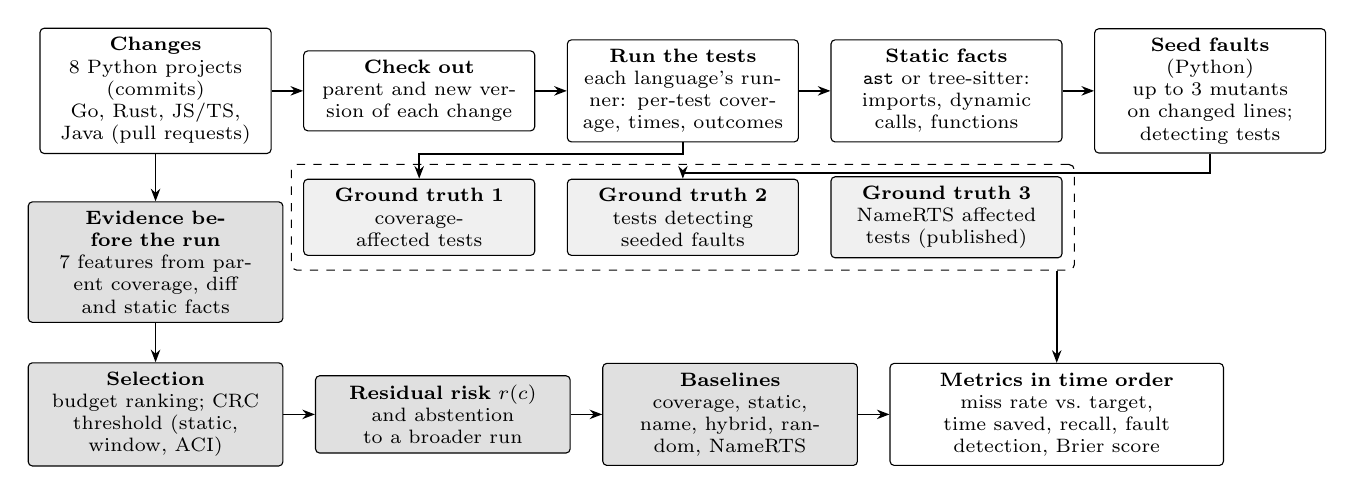
\begin{tikzpicture}[font=\scriptsize, node distance=3.5mm and 4mm,
  box/.style={draw, rounded corners=1.5pt, align=center, minimum height=9mm, text width=27mm, fill=white},
  gt/.style={box, fill=black!6}, an/.style={box, text width=30mm, fill=black!12},
  arr/.style={-{Stealth[length=1.6mm]}, semithick}]
\node[box] (hist) {\textbf{Changes}\\ 8 Python projects (commits)\\ Go, Rust, JS/TS, Java (pull requests)};
\node[box, right=of hist] (co) {\textbf{Check out}\\ parent and new version of each change};
\node[box, right=of co] (run) {\textbf{Run the tests}\\ each language's runner: per-test coverage, times, outcomes};
\node[box, right=of run] (st) {\textbf{Static facts}\\ \texttt{ast} or tree-sitter: imports, dynamic calls, functions};
\node[box, right=of st] (mut) {\textbf{Seed faults} (Python)\\ up to 3 mutants on changed lines; detecting tests};
\node[gt, below=6mm of co] (g1) {\textbf{Ground truth 1}\\ coverage-affected tests};
\node[gt, right=of g1] (g2) {\textbf{Ground truth 2}\\ tests detecting seeded faults};
\node[gt, right=of g2] (g3) {\textbf{Ground truth 3}\\ NameRTS affected tests (published)};
\node[an, below=6mm of hist] (f) {\textbf{Evidence before the run}\\ 7 features from parent coverage, diff and static facts};
\node[an, below=5mm of f] (sel) {\textbf{Selection}\\ budget ranking; CRC threshold (static, window, ACI)};
\node[an, right=of sel] (risk) {\textbf{Residual risk} $r(c)$\\ and abstention to a broader run};
\node[an, right=of risk] (base) {\textbf{Baselines}\\ coverage, static, name, hybrid, random, NameRTS};
\node[box, right=of base, text width=40mm] (met) {\textbf{Metrics in time order}\\ miss rate vs.\ target, time saved, recall, fault detection, Brier score};
\draw[arr] (hist) -- (co); \draw[arr] (co) -- (run); \draw[arr] (run) -- (st); \draw[arr] (st) -- (mut);
\draw[arr] (run.south) -- ++(0,-1.5mm) -| (g1.north);
\draw[arr] (mut.south) |- ++(0,-2.5mm) -| (g2.north);
\draw[arr] (hist.south) -- (f.north);
\draw[arr] (f) -- (sel); \draw[arr] (sel) -- (risk); \draw[arr] (risk) -- (base); \draw[arr] (base) -- (met);
\node[draw, dashed, rounded corners=2pt, inner sep=1.5mm, fit=(g1)(g2)(g3)] (gts) {};
\draw[arr] (gts.south -| met.north) -- (met.north);
\end{tikzpicture}%
}
\caption{Study workflow. The collection steps (top row) run on GitHub Actions in 52 parallel shards. The analysis (bottom row) processes each project's changes in time order and uses the test run of the new version only to build the ground truths. The multi-language replication (Section~6.7 of the article) follows the same steps on pull requests inside the benchmark's Docker images, without seeded faults.}
\label{fig:workflow}
\end{figure}

\section*{S4\quad Additional results}
Fig.~\ref{fig:budget} belongs to RQ1 (budget mode), Figs.~\ref{fig:perproject}, \ref{fig:reliability} and~\ref{fig:calib} to RQ2, Fig.~\ref{fig:triggers} to RQ3, Fig.~\ref{fig:languages} to RQ6 and Table~\ref{tab:ablation} to the ablation of the article.

\begin{figure}[htbp]
\centering
\includegraphics[width=\linewidth]{figures/budget.pdf}
\caption{Recall of affected tests at different time budgets (history projects).}
\label{fig:budget}
\end{figure}

\begin{figure}[htbp]
\centering
\includegraphics[width=\linewidth]{figures/per_project.pdf}
\caption{Share of changes with a missed affected test per project at target $\alpha=0.10$ ($^\ast$NameRTS commits). A bar of zero means no miss.}
\label{fig:perproject}
\end{figure}

\begin{figure}[htbp]
\centering
\includegraphics[width=\linewidth]{figures/reliability.pdf}
\caption{Reliability of the residual-risk estimate $r(c)$ (history projects): mean estimate against observed miss rate in five bins; numbers give the changes per bin. Points below the diagonal overestimate the risk.}
\label{fig:reliability}
\end{figure}

\begin{figure}[htbp]
\centering
\includegraphics[width=\linewidth]{figures/triggers.pdf}
\caption{Share of unsafe and of safe changes (for line-coverage selection) that each abstention rule flags (history projects). A useful rule flags many unsafe and few safe changes.}
\label{fig:triggers}
\end{figure}

\begin{figure}[htbp]
\centering
\includegraphics[width=\linewidth]{figures/calibration.pdf}
\caption{Observed miss rate against the target $\alpha$ for the three calibration variants (history projects). Points below the dotted line meet the target.}
\label{fig:calib}
\end{figure}

\begin{figure}[htbp]
\centering
\includegraphics[width=\linewidth]{languages.pdf}
\caption{Observed miss rate against the target $\alpha$ for a threshold calibrated once (left) and for adaptive calibration (right), on the Python history projects and on the Go, Rust and JavaScript/TypeScript pull requests (test changes). Points on the dashed line meet the target exactly.}
\label{fig:languages}
\end{figure}

\begin{table}[htbp]
\caption{Ablation of evidence signals (25\% budget, history projects)}
\label{tab:ablation}
\centering
\footnotesize
\begin{tabular}{@{}lrrrr@{}}
\toprule
\textbf{Model} & \textbf{Recall} & \textbf{Safe\%} & \textbf{Mut.\%} & \textbf{$\Delta$Recall} \\
\midrule
Full model & 0.655 & 34.6 & 91.1 & -- \\
$-$ co-change & 0.655 & 34.6 & 91.1 & +0.000 \\
$-$ name match & 0.655 & 34.6 & 91.1 & +0.000 \\
$-$ static import & 0.654 & 34.6 & 91.1 & -0.000 \\
$-$ function coverage & 0.654 & 34.6 & 91.1 & -0.000 \\
$-$ test changed & 0.654 & 34.6 & 91.1 & -0.001 \\
$-$ file coverage & 0.650 & 34.3 & 91.4 & -0.004 \\
$-$ line coverage & 0.647 & 34.3 & 90.5 & -0.008 \\
$-$ all coverage & 0.601 & 30.1 & 90.8 & -0.054 \\
\bottomrule
\end{tabular}
\end{table}

\bibliographystyle{unsrtnat}
\bibliography{refs}
\end{document}
